\documentclass[11pt, oneside]{article}   	% use "amsart" instead of "article" for AMSLaTeX format


%\usepackage{draftwatermark}
% \SetWatermarkText{Confidential}
% \SetWatermarkScale{5}
% \SetWatermarkLightness {0.85} 
% \SetWatermarkColor[rgb]{0.7,0,0}


\usepackage{geometry}                		% See geometry.pdf to learn the layout options. There are lots.
\geometry{letterpaper}                   		% ... or a4paper or a5paper or ... 
%\geometry{landscape}                		% Activate for for rotated page geometry
%\usepackage[parfill]{parskip}    		% Activate to begin paragraphs with an empty line rather than an indent
\usepackage{graphicx}				% Use pdf, png, jpg, or eps� with pdflatex; use eps in DVI mode
								% TeX will automatically convert eps --> pdf in pdflatex		
\usepackage{amssymb}
\usepackage{mathrsfs}
\usepackage{hyperref}
\usepackage{url}
\usepackage{subcaption}
\usepackage{authblk}
\usepackage{amsmath}
\usepackage{mathtools}
\usepackage{graphicx}
\usepackage{fixltx2e}
\usepackage{hyperref}
\usepackage{alltt}
\usepackage{color}
\usepackage[utf8]{inputenc}
\usepackage[english]{babel}
 
\newtheorem{theorem}{Theorem}[section]
\newtheorem{corollary}{Corollary}[theorem]
\newtheorem{lemma}[theorem]{Lemma}

\newcommand{\argmax}{\operatornamewithlimits{argmax}}
\newcommand{\argmin}{\operatornamewithlimits{argmin}}



\title{A Few Notes on Fisher Information (WIP)}
\author{David Meyer \\ dmm@\{1-4-5.net,uoregon.edu\}}

\date{Last update: \today}							% Activate to display a given date or no date


\begin{document}
\maketitle

\section{Definitions} 
\label{sec:defs}
There are so many interesting things about Fisher Information \cite{2017arXiv170501064L} and its theoretical properties (and for that matter, its applications), but I'll
start here with definitions.  Let $\{P_{\theta}\}_{\theta \in \Theta}$ denote a parametric family of distributions on a space $\mathcal{X}$, where each 
$\theta \in \Theta \subset \mathbb{R}^d$ indexes  $\{P_{\theta}\}$.  Assume (with no real loss of generality, AFAICT) that each $P_\theta$  has a density $p_\theta$. 
Then the Fisher information associated with the \emph{model} is the matrix given by

\begin{flalign}
\mathbb{I}_{\theta} \coloneqq \mathbb{E}_{\theta} \Big [\nabla_{\theta} \log p_{\theta}(X) \nabla_{\theta} \log p_{\theta}(X)^{\small{\text{T}}} \Big] =
\mathbb{E}_{\theta} [l_{\theta}l_{\theta}^T]
\end{flalign}
where $l_\theta$ is the \emph{score function} $\nabla_{\theta} \log p_{\theta}(X)$. The score function turns up in perhaps unexpected places (e.g., score function gradient in policy gradient reinforcement learning) and has various applications.

\bigskip
\noindent
Essentially the Fisher Information tells us how much information a random variable $\mathcal{X}$ contains about the parameter vector $\theta$, where 
$\mathcal{X}$ is distributed according to a probability distribution parameterized by $\theta$. Intuitively, the Fisher information captures the variability of
 the gradient of the score function, $\nabla_\theta \log p_\theta(x)$; in a family of distributions for which the score function has high variability, we expect 
 estimation of the parameter $\theta$ to be easier; essentially (and perhaps counter-Intuitively) events with lower probability contain more information.

\bigskip
\noindent
Fisher Information can be described in various ways. One way to think about the Fisher Information is that it is the variance of the score function $l_\theta$. Recall that the mean $\mu = \mathbb{E}[X]$ and the variance $\sigma^2 = \mathbb{E}[(X - \mu)^2]$. First, consider 
$\mathbb{E}\big[\nabla_{\theta} \log p_{\theta}(X)\big] = \mathbb{E}\big[l_\theta\big]$. 

\begin{flalign}
\mathbb{E}_{\theta}\big [l_\theta\big] & = \int p_{\theta}(x) \nabla_{\theta} \log p_{\theta}(x) dx  \;  \qquad \qquad \mathrel{\#} \text{Definition of Expectation} \\
&= \int \frac{\nabla_\theta p_\theta(x)}{p_\theta(x)} p_\theta(x) dx  \; \; \quad  \qquad \qquad \mathrel{\#} \nabla_{\theta} \log p_{\theta}(x)  
= \frac{\nabla_{\theta} p_\theta(x)}{p_\theta(x)} \\
&= \int \nabla_\theta p_\theta(x) dx  \quad \qquad  \qquad  \quad \qquad \mathrel{\#} \frac{p_\theta(x)}{p_\theta(x)} = 1 \\
&= \nabla_\theta \int p_\theta(x) dx  \qquad \qquad  \qquad \qquad \mathrel{\#} \text{Assume $\int$ and $\nabla$ can be exchanged} \\
&= \nabla_{\theta} 1 \; \qquad \qquad  \qquad \qquad  \qquad \qquad \mathrel{\#}  \text{$p_\theta(x)$  is a density so} \int_x p_\theta(x) dx = 1 \\
&= 0  \; \; \quad  \qquad \qquad \qquad \qquad \qquad \qquad \mathrel{\#} \text{for c any constant } \nabla c = 0
\end{flalign}

\bigskip
\noindent
So the mean $\mu$ of the score function, $\mathbb{E}_{\theta}\big[\nabla_{\theta} \log p_{\theta}(X)\big]  = 0$. This condition (expected value is zero) is the  \emph{regularity condition} required by the Cram\'er Rao Bound. See Section \ref{sec:crlb} for more on the Cram\'er Rao Bound (sometimes Cram\'er Rao Lower Bound or CRLB).

\bigskip
\noindent
Now, recall that the variance $\sigma^2 = \mathbb{E}[(X - \mu)^2]$. However, we know that $\mathbb{E}_{\theta}\big [l_\theta\big] = 0$, so 
$\mathbb{I}_\theta = \text{Var}(l_\theta) = \mathbb{E} \big [\big (\nabla_\theta \log p_\theta(x)\big)^2 \big ]$. Under relatively mild conditions
($\frac{\partial^2}{\partial {\theta}} p_\theta(x)$ exists) and using the chain rule we see that

\begin{flalign}
\nabla_{\theta}^{2} \log p_\theta(x) &= \frac{\nabla_{\theta}^{2}  p_\theta(x)}{p_\theta(x)} - \frac{\nabla_\theta p_\theta(x) \nabla_\theta p_\theta(x)^{\small{T}}}{{p_\theta(x)^2}}
 \quad  \qquad \qquad \mathrel{\#} \text{ finite differences}\\
&= \frac{\nabla_{\theta}^{2}  p_\theta(x)}{p_\theta(x)} - \nabla_\theta \log p_\theta(x) \nabla_\theta \log p_\theta(x)^{\small{T}}  \qquad \mathrel{\#} \nabla_{\theta} \log p_{\theta}(x)  = \frac{\nabla_{\theta} p_\theta(x)}{p_\theta(x)} \\
&= \frac{\nabla_{\theta}^{2}  p_\theta(x)}{p_\theta(x)} - l_\theta l_{\theta}^{\small{T}} \: \quad \qquad \qquad \qquad \qquad \qquad \mathrel{\#} \text{ definition of } l_\theta \\
l_\theta l_{\theta}^{\small{T}}  &= -\nabla_{\theta}^{2} \log p_\theta(x) + \frac{\nabla_{\theta}^{2}  p_\theta(x)}{p_\theta(x)} \; \;\:  \:\qquad \qquad \qquad  \mathrel{\#} \text{ algebra}
\label{eqn:llt}
\end{flalign}




\bigskip
\noindent
So far we have the following forms of the Fisher Information $\mathbb{I}_\theta$:
 \begin{flalign}
\mathbb{I}_\theta = \text{Var}(l_\theta)   = \mathbb{E}_{\theta} \big [ l_\theta l_{\theta}^{\small{\text{T}}} \big ] =  \mathbb{E} \big [\big (\nabla_\theta \log p_\theta(x)\big)^2 \big ]
\end{flalign}

\bigskip
\noindent
It turns out that using Equation \ref{eqn:llt} we can see that  $\mathbb{I}_\theta$  also turns out to equal $ -\mathbb{E}_{\theta} \big [\nabla^2 \log p_\theta(x) \big] $, 
which we can see as follows:

\begin{flalign}
\mathbb{I}_\theta 
&= \mathbb{E}_{x \sim p_\theta(x)} \big [l_\theta l_\theta^{\small{T}} \big ] 
\; \:\qquad \qquad \qquad \qquad \qquad \qquad \qquad \qquad \qquad \mathrel{\#} \text{ definition of } \mathbb{I}_\theta \\
&= \mathbb{E}_\theta \Bigg [ - \nabla_{\theta}^{2} \log p_\theta(x) + \frac{\nabla_{\theta}^{2}  p_\theta(x)}{p_\theta(x)} \Bigg ] 
\quad \qquad \qquad \qquad \qquad \qquad \mathrel{\#} \text{ Equation \ref{eqn:llt}} \\
&= - \int p_\theta(x) \nabla^2 \log p_\theta(x) dx + \int \frac{p_\theta(x) \nabla^2 p_\theta(x) dx}{p_\theta(x)}
\;\; \qquad \qquad \mathrel{\#} \text{ Defn Expectation}\\
&= - \int p_\theta(x) \nabla^2 \log p_\theta(x) dx + \int \nabla^2 p_\theta(x) dx 
\quad \qquad \qquad \qquad \mathrel{\#} \frac{p_\theta(x)}{p_\theta(x)} = 1\\
&= -\mathbb{E}_{\theta} \big [\nabla^2 \log p_\theta(x) \big] + \nabla^2 \underbrace{\int p_\theta(x) dx}_{1} 
\label{eqn:int21}
\; \: \quad \qquad \qquad \qquad \qquad \mathrel{\#} p_\theta(x) \text{ is a density} \\
&=  -\mathbb{E}_{\theta} \big [\nabla^2 \log p_\theta(x) \big] + \nabla^2 1 
\;\;\; \quad \qquad \qquad \qquad \qquad \qquad \qquad \mathrel{\#} \text{ Equation \ref{eqn:int21}} \\
&=  -\mathbb{E}_{\theta} \big [\nabla^2 \log p_\theta(x) \big] + 0 
\; \; \;\;\qquad  \qquad \qquad \qquad \qquad \qquad \qquad \mathrel{\#}  \nabla c = 0  
\label{eqn:nabla} \\
&=  -\mathbb{E}_{\theta} \big [\nabla^2 \log p_\theta(x) \big] 
\end{flalign}
\noindent
where the $c$ in Equation \ref{eqn:nabla} is any constant.

\bigskip
\noindent
So in summary, we know that that the Fisher Information $\mathbb{I}_\theta$ equals

\begin{flalign}
\mathbb{I}_\theta = \mathbb{E}_\theta \big [ l_\theta l_{\theta}^{\small{T}} \big ] =  -\mathbb{E}_{\theta} \big [\nabla^2 \log p_\theta(x) \big]
\end{flalign}

\bigskip
\noindent
This representation also makes clear the additional fact that, if we have $n$ i.i.d. observations from the model $P_\theta$ then the information content 
 grows linearly, that is, $\log p_\theta(X_1^n) = \sum\limits_{i=1}^n \log p_\theta(X_i)$.

\bigskip
\noindent
Perhaps surprisingly, $\mathbb{I}_\theta$ also equals $\mathrm{Cov}_x \big [\nabla_\theta \log p_\theta(x) \big ]$, which we'll see in Section \ref{sec:crlb}. 
But there's more. The Fisher Information is related to the KL-divergence, as follows:

\begin{flalign}
\mathbb{I}_\theta = \nabla^2_{\theta^\prime} D_{\text{KL}} (p_{\theta^\prime} (x) \mid \mid p_{\theta}(x))  = 
 \nabla^2_{\theta^\prime} D_{\text{KL}} (p_\theta (x) \mid \mid p_{\theta^\prime} (x))
\end{flalign}

\bigskip
\noindent
It is unusual for the KL to be symmetrical in this way. We will see more about this in Section \ref{sec:estimation}.

\section{Estimation and Fisher information}
\label{sec:estimation}
The Fisher information has intimate connections to estimation, both in terms of classical estimation and various "information games".  The canonical motivating example 
appears to be estimation of the mean of a sample of $n$ i.i.d.  $X_1^n \sim \mathrm{Bernoulli}(p), p \in [0,1]$.  The standard formulation of the Bernoulli probability mass function (pmf)  $f$  for $x \in [0,1]$ looks like 
\begin{flalign}
f(x;p) &=
  \begin{cases}
    p     & \text{if $x = 1$}, \\
    1 - p & \text{if $x = 0$}.
  \end{cases} \\
  &= p^{x}(1-p)^{1-x}
\end{flalign}
So if we take the pmf of the Bernoulli distribution to be $P(X = x) =  p^{x}(1-p)^{1-x}$, then $\nabla P(X = x) = \frac{x}{p} - \frac{1-x}{1-p}$, so that
\begin{flalign}
\mathbb{I}_p &= \mathbb{E}_p \Bigg [\Bigg (\frac{X}{p} - \Bigg(\frac{1-X}{1-p} \Bigg) \Bigg)^2\Bigg] \\
&=\frac{1}{p} + \frac{1}{1 - p} \\
& = \frac{1}{p (1-p)}
\label{eqn:fisher}
\end{flalign}

\noindent
where $\mathbb{I}_p$ is the Fisher Information for  a single sample.

\bigskip
\noindent
The variance of a Bernoulli distribution with sample mean $\mu$ looks like this: 
\begin{flalign}
\mathbb{E}\big [(X- \mu)^2 \big] &= \frac{1}{n} \mathrm{Var}(X)  \qquad \qquad \mathrel{\#}  \mu = p \text{ (Bernoulli disribution})\\
&= \frac{p(1-p)}{n} \; \qquad \qquad \mathrel{\#} \text{Variance of the Bernoulli distribution} \\
&= \frac{1}{\mathbb{I}_p} \cdot \frac{1}{n} \: \; \quad \qquad \qquad \mathrel{\#} p(1-p) = \frac{1}{\mathbb{I}_p}, \text{ Equation } \ref{eqn:fisher} \\
\text{Var}(X) &=\frac{1}{\mathbb{I}_{\theta}}
\label{eqn:inverse}
\end{flalign}

\bigskip
\noindent
It turns out that this inverse dependence of the variance on Fisher Information (Equation \ref{eqn:inverse}) is unavoidable, and is 
quantified by the Cram\'er Rao Bound, which provides lower bounds on the mean squared error of all unbiased estimators.

\section{The Cram\'er Rao Lower Bound}
\label{sec:crlb}
The Cram\'er Rao Lower Bound (CRLB) answers the question: Given an estimation problem, what is the variance of the best possible estimator? 

\subsection{Brief Review of Terms}
By way of review, recall that a \emph{statistic} is a single measure of some attribute of a sample (e.g., its arithmetic mean value). It is calculated by applying a function 
(statistical algorithm) to the values of the items of the sample, which are known together as a set of data. So suppose we have a sample $D= X_1^n$ then 
$f:D \rightarrow \mathbb{R}$ is a \emph{statistic on $D$}. Statistics have all kinds of interesting properties that we won't review here, including observability\footnote{A statistic is an observable random variable, which differentiates it both from a parameter that is a generally unobservable quantity describing a property of a statistical population, and from an unobservable random variable, such as the difference between an observed measurement and a population average, that is., $\frac{1}{n} \sum\limits_{i = 1}^n X_i - \mu$, where 
the $X_i$ are the observations and $\mu$ is the true population mean.}
completeness, consistency, sufficiency, unbiasedness.
Other examples of properties of a statistic include minimum mean square error, low variance, robustness, and computational convenience, and measures of information such 
as the Fisher Information.

\bigskip
\noindent
An \emph{estimator} is a rule for calculating an estimate of a statistic based on observed data. An estimator is usually described in terms of an (unknown) parameter
$\theta$.  So an "estimator" or "point estimate" is a statistic (that is, a function of the data, e.g., $f$ above) that is used to infer the value of an unknown parameter in a 
statistical model. The parameter being estimated is sometimes called the estimand. It can be either finite-dimensional (in parametric and semi-parametric models), or 
infinite-dimensional (semi-parametric and non-parametric models). In any cases the parameter is denoted $\theta$  and the estimator is traditionally 
written by adding a circumflex over the symbol: $\widehat {\theta}$. Being a function of the data, the estimator is itself a random variable; 
a particular realization of this random variable is called the "estimate", the words "estimator" and "estimate" are used interchangeably.

\bigskip
\noindent
An example of an estimator is the \emph{bias}: The bias of  an estimator $\widehat {\theta }$  is defined as  $\text{Bias}(\widehat{\theta}) = \mathbb{E} [\widehat {\theta}] - \theta$.  
It is the distance  between the average of the collection of estimates and the true value of the parameter being estimated. Note that the bias of $\widehat{\theta}$ is a 
function of the  true value of  $\theta$  so saying that the bias of $\widehat{\theta}$ is $b$ means that for every $\theta$  the bias of  $\widehat{\theta}$  is $b$. 
An \emph{unbiased} estimator has the property that $\mathbb{E} [\widehat {\theta}]  = \theta$, that is, $\text{Bias}(\widehat{\theta}) = 0$. Note that interestingly, the 
\emph{Mean Squared Error} (MSE) of a sample, its variance, and its bias, are related
in particular, 
$\text{MSE} (\widehat {\theta})=\text{Var}(\widehat {\theta}) + \text{Bias}(\widehat {\theta})^2$, That is, the MSE = Variance + square of the Bias. This suggests the important 
result that for an unbiased estimator $\widehat{\theta}$, $ \text{Var}(\widehat {\theta}) = \text{MSE} (\widehat {\theta})$. You can show this pretty easily:

\begin{flalign}
\text{MSE}(\widehat{\theta}) &= \mathbb{E} \big [(\theta - \widehat{\theta})^2 \big] \\
&= \mathbb{E} \big [( \theta - \mathbb{E}[\widehat{\theta}] +  \mathbb{E}[\widehat{\theta}] - \widehat{\theta})^2 \big ] \\
&=  \mathbb{E} \big [(\theta - \mathbb{E}[\widehat{\theta}])^2  + \mathbb{E} \big [(\mathbb{E}[\widehat{\theta}] - \widehat{\theta})^2 \big ] +
\mathbb{E} \big [(2(\theta - \mathbb{E}[\widehat{\theta}])(\mathbb{E}[(\widehat{\theta}] - \widehat{\theta})\big ] \\
&= \mathbb{E} \big [\underbrace{(\theta - \mathbb{E}[\widehat{\theta}])^2}_{\text{Bias}(\widehat{\theta})^2} \big ]  + 
\mathbb{E} \big [\underbrace{(\mathbb{E}[\widehat{\theta}] - \widehat{\theta})]^2}_{\text{Var}(\widehat{\theta})} \big ]+
\underbrace{2(\theta - \mathbb{E}[\widehat{\theta}]) (\mathbb{E}[\widehat{\theta}] - \mathbb{E}[\widehat{\theta}])}_{\mathbb{E}[\widehat{\theta}] - \mathbb{E}[\widehat{\theta}] \; = \;  0} \\
\text{MSE}(\widehat{\theta}) &= \text{Bias}(\widehat{\theta})^2 + \text{Var}(\widehat{\theta})
\end{flalign}

\bigskip
\noindent
Of course, if $\text{Bias}(\widehat{\theta}) = 0$ ($\widehat{\theta}$ is unbiased), then $\text{MSE}(\widehat{\theta})  = \text{Var}(\widehat{\theta})$.

\bigskip
\noindent
Back to the CRLB. Recall that the question at had was given an estimation problem, what is the variance of the best possible estimator?
The CRLB gives and answer to this question, as well as a somewhat impractical method for finding the best estimator.  To get some intuition about the 
CRLB, consider the the problem of estimating the DC level A in the model
\begin{flalign}
x[n] = \text{A} + w[n]
\end{flalign}
\noindent 
where the signal we are looking for is embedded in the White Gaussian Noise (WGN) $w[n] \sim \mathcal{N}(0,\sigma^2)$.
For simplicity, suppose that we are using only a single observation to do this, and let this observation be $x[0]$. Then the pdf of
$x[0]$ is Gaussian:

\begin{flalign}
p(x[n];A) =  \frac{1}{\sqrt{2 \pi \sigma^2}} \exp{\Bigg [ - \frac{1}{2 \sigma^2} (x[0] - \text{A})^2\Bigg ]}
\label{eqn:likelihood}
\end{flalign}

\bigskip
\noindent
One we observe some value of $x[0]$, say $x[0] = 3$, some values of A become more likely. In fact, the pdf of A has the same 
form as the pdf of $x[0]$.

\begin{flalign}
p(A) =  \frac{1}{\sqrt{2 \pi \sigma^2}} \exp{\Bigg [ - \frac{1}{2 \sigma^2} (x[0] - 3)^2\Bigg ]}
\end{flalign}

\bigskip
\noindent
Figure \ref{fig:pdfs} shows the pdf plotted for $\text{A} = 3$ and $\sigma^2 = \frac{1}{3}$ and $\sigma^2 = 1$. The main observation
here is that that we will probably get more accurate results for the pdf in the upper case, but why? Before answering this question, 
here are a few observations

\begin{itemize}
\item  When the pdf is viewed as a function of the unknown parameter $\theta$ and with $x[.]$ fixed.
the pdf is called the \emph{likelihood function}.
\item The curvature of the likelihood function determines how accurately we can estimate the parameter. 
For example, for the pdf on top in Figure \ref{fig:pdfs} it is easier to estimate $\theta$.  In fact,  if a single sample is observed
as $x[0] = \text{A} + w[0]$, then we can expect a better estimate if $\sigma^2$ is small.
\end{itemize}

\bigskip
\noindent
But still, \emph{why} should we expect a better estimate where $\sigma^2$ is small, and can we quantify this effect?
Further, is there any measure that would be common for all possible estimators for a specific estimation problem?
Specifically, we?d like to find the smallest possible variance.  We know that the second derivative of the likelihood 
function (or log-likelihood) is one alternative for measuring the curvature of a function, so this is a good candidate. Let's 
see what happens in this case. BTW, what this is saying in some sense is that the minimum variance 
$\sigma^2_{\text{min}} = - \frac{1}{curvature}$. 


\begin{figure}
\center{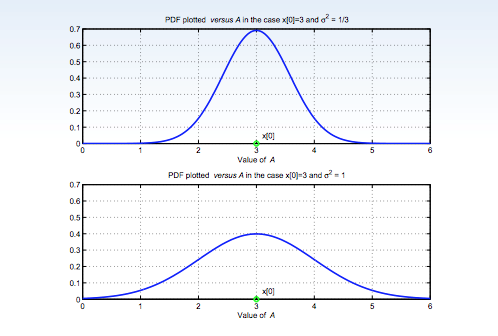
\includegraphics[scale=1.5] {images/pdf}}
\caption{pdfs for $\text{A} = 3$, and  $\sigma^2 = 1/3$  and $\sigma^2 = 1$}
\label{fig:pdfs}
\end{figure}

\bigskip
\noindent
First, notice that in this case the minimum variance of all estimators is $\sigma^2$ since
we are using only one sample. We also know that the likelihood function; this is given in Equation \ref{eqn:likelihood}. Given this 
likelihood, the log-likelihood is 
\begin{flalign}
\ln p(x[0];\text{A}) = - \ln \sqrt{2\pi\sigma^2} - \frac{1}{2\sigma^2} (x[0] - A)^2
\end{flalign}

\bigskip
\noindent
The derivative with respect A to a is given by

\begin{flalign}
\frac{\partial \ln p(x[0];\text{A})}{\partial \text{A}} = \nabla_{\tiny{\text{A}}} \ln p(x[0];\text{A}) = \frac{1}{\sigma^2}(x[0] - \text{A})
\end{flalign}

\bigskip
\noindent
and the second derivative is
\begin{flalign}
\frac{\partial^2 \ln p(x[0];\text{A})}{\partial^2 \text{A}} = \nabla^2_{\text{A}} \ln p(x[0];\text{A}) = -  \frac{1}{\sigma^2}
\end{flalign}

\bigskip
\noindent
Since $\sigma^2$ is the smallest possible variance, in this case we have an alternative way of finding the minimum variance
of all estimators, in paricular
\begin{flalign}
\sigma^2_{\text{min}} = - \frac{1}{\frac{\partial^2 \ln p(x[0];\text{A})}{\partial^2 \text{A}}} = - \frac{1}{\text{curvature of the likelihood}}
\end{flalign}

In order to generalize the result, the following regularity conditions must hold:
\begin{itemize}
\item If the function depends on the data $X$, you must take the expectation with respect to $X$
\item If the function depends on the parameter $\theta$, then evaluate the  derivative at the true value of $\theta$
\end{itemize}

\bigskip
\noindent
All of this put together gives us the Minimum Variance Unbiased Estimator (MVUE):
 
\begin{equation*}
\text{MVUE} = \frac{1}{- \mathbb{E} \Big [\frac{\partial^2 \ln p(x[0]; \theta)}{\partial^2 \theta} \Big ] }
\end{equation*}


\subsection{CRLB Scalar Parameter}

\textbf{Theorem:  CRLB Scalar Parameter Case} 

\bigskip
\noindent
Assuming that the pdf $p(x;\theta)$ satisfies the regularity condition that 
$\forall \theta$,  \\
$\mathbb{E}_{x \sim p(x;\theta)} \Big [ \frac{\partial \ln p(x; \theta)}{\partial \theta} \Big ] = 0$, then the \emph{variance} of any unbiased
estimator $\widehat{\theta}$ must satisfy

\begin{equation}
\text{Var}(\widehat{\theta}) \geqslant \frac{1}{- \mathbb{E} \Big [\frac{\partial^2 \ln p(x; \theta)}{\partial^2 \theta} \Big ]}
\end{equation}

\bigskip
\noindent
An important consequence of  the Theorem is that any unbiased estimator can attain this lower bound $\forall \theta$ if and only if 
\begin{equation}
\label{eqn:crlb1}
\frac{\partial \ln p(x;\theta)}{\partial \theta} = \mathbb{I}_{\theta}(g(x) - \theta)
\end{equation}
\noindent
for some functions $g$ and $\mathbb{I}$. That estimator, which is the MVUE
has $\widehat{\theta} = g(x)$ with minimum variance is $\frac{1}{\mathbb{I}_\theta}$. The proof of Equation \ref{eqn:crlb1} can be found in 
\cite{Kay:1993:FSS:151045} and elsewhere around the web.

\bigskip
\noindent
\textbf{Notes on the CRLB Scalar Parameter Case}
\begin{itemize}
\item Note that the Fisher Information $\mathbb{I}_\theta =  \mathbb{E} \Big [\frac{\partial^2 \ln p(x; \theta)}{\partial^2 \theta} \Big ]$
so that by the Theorem:  \\
$\text{Var}(\widehat{\theta}) \geqslant \mathbb{I}_\theta^{-1}$.
\item The CRLB provides a lower bound for an estimator's error variance
\item  We need to know the pdf to evaluate CRLB. Often we don?t know this information and cannot evaluate this bound. OTOH,
if the data is multivariate Gaussian or i.i.d. with known distribution then we can find the CRLB.
\item If the estimator reaches the CRLB, it is called \emph{efficient}.
\item The MVUE may or may not be efficient, and it is not guaranteed that MVUE exists or even is realizable.
\end{itemize}

\subsection{Example: Estimation of the DC Level in WGN}
\label{subsec:wgn}

Consider the DC level in White Gaussian Noise with $N$ data points: $x[n] = A + w[n], n = 0, 1,  \hdots, N-1$. The question we want to answer
is:  What is the minimum variance of any unbiased estimator using N samples? Recall that the pdf and the likelihood function are both  the product of
the individual densities so that
\begin{flalign}
p(x;A) &= \prod\limits_{n = 0}^{N - 1} \frac{1}{\sqrt{2 \pi \sigma^2}} \exp{\Big [ - \frac{1}{2 \sigma^2} (x[n] -A)^2 }\Big ] \\
&= \frac{1}{(2 \pi \sigma^2)^{\frac{N}{2}}} \exp{\Big [- \frac{1}{2 \sigma^2} \sum\limits_{n=0}^{N-1} (x[n] - A)^2} \Big ]
\end{flalign}

\bigskip
\noindent
The log-likelihood is now
\begin{flalign}
\ln p(x;A) &= -\ln \big [(2 \pi \sigma^2)^{\frac{N}{2}} \big] - \frac{1}{2 \sigma^2} \sum\limits_{n=0}^{N-1} (x[n] - A)^2
\end{flalign}

\bigskip
\noindent
and the first derivative is 
\begin{flalign}
\frac{\partial \ln p(x;A)}{\partial A} &= \frac{1}{\sigma^2} \sum\limits_{n=0}^{N-1} (x[n] - A) \\
&= \frac{N}{\sigma^2} (\tilde{\textbf{x}} - A)
\end{flalign}
\noindent
where $\tilde{\textbf{x}}$ is the sample mean. The second derivative has the simple form

\begin{flalign}
\frac{\partial^2 \ln p(x;A)} {\partial A^2} &= - \frac{N}{\sigma^2} 
\end{flalign}

\bigskip
\noindent
hence the minimum variance of any \emph{unbiased} estimator is 
\begin{flalign}
\text{Var}(\hat{A}) \geqslant   \frac{N}{\sigma^2} 
\end{flalign}

\bigskip
\noindent
\textbf{Theorem:  CRLB Vector Parameter Case} 

\bigskip
\noindent
It is again assumed that the pdf $p(x;\theta)$ satisfies the \emph{regularity} conditions as above.  Then the covariance matrix of any unbiased estimator 
$\widehat{\theta}$ not surprisingly satisfies

\begin{flalign}
\textbf{C}_{\widehat{\theta}} - \mathbb{I}^{-1}_\theta \geqslant 0
\end{flalign}

\noindent
where $\geqslant$ is interpreted as \emph{positive semidefinite}. Here the Fisher Information matrix is given by

\begin{flalign}
\big [ \mathbb{I}_\theta \big ]_{ij} = -  \mathbb{E}_{x \sim p(x; \theta)}  \Bigg [ \frac{\partial \ln p(x;\theta)}{\partial \theta_i \partial \theta_j} \Bigg ]
\end{flalign}
\noindent
Furthermore, an unbiased estimator may be found that attains the bound in that $\textbf{C}_{\widehat{\theta}} = \mathbb{I}^{-1}_{\theta}$ \emph{iff}

\begin{flalign}
\frac{\partial \ln p(x;\theta)}{\partial \theta} = \mathbb{I}_{\theta}(g(x) - \theta)
\end{flalign}
\noindent
for some function $g$ and some $m \times m$ matrix $\mathbb{I}_{\theta}$. That estimator, which s the MVUE, is given by $\widehat{\theta} = g(x)$ and the 
covariance matrix is $\mathbb{I}^{-1}_{\theta}$.

\newpage
\bibliographystyle{ieeetr}
\bibliography{/Users/dmm/papers/bib/ml}



\end{document} 
